% Options for packages loaded elsewhere
\PassOptionsToPackage{unicode}{hyperref}
\PassOptionsToPackage{hyphens}{url}
%
\documentclass[
]{article}
\usepackage{lmodern}
\usepackage{amssymb,amsmath}
\usepackage{ifxetex,ifluatex}
\ifnum 0\ifxetex 1\fi\ifluatex 1\fi=0 % if pdftex
  \usepackage[T1]{fontenc}
  \usepackage[utf8]{inputenc}
  \usepackage{textcomp} % provide euro and other symbols
\else % if luatex or xetex
  \usepackage{unicode-math}
  \defaultfontfeatures{Scale=MatchLowercase}
  \defaultfontfeatures[\rmfamily]{Ligatures=TeX,Scale=1}
\fi
% Use upquote if available, for straight quotes in verbatim environments
\IfFileExists{upquote.sty}{\usepackage{upquote}}{}
\IfFileExists{microtype.sty}{% use microtype if available
  \usepackage[]{microtype}
  \UseMicrotypeSet[protrusion]{basicmath} % disable protrusion for tt fonts
}{}
\makeatletter
\@ifundefined{KOMAClassName}{% if non-KOMA class
  \IfFileExists{parskip.sty}{%
    \usepackage{parskip}
  }{% else
    \setlength{\parindent}{0pt}
    \setlength{\parskip}{6pt plus 2pt minus 1pt}}
}{% if KOMA class
  \KOMAoptions{parskip=half}}
\makeatother
\usepackage{xcolor}
\IfFileExists{xurl.sty}{\usepackage{xurl}}{} % add URL line breaks if available
\IfFileExists{bookmark.sty}{\usepackage{bookmark}}{\usepackage{hyperref}}
\hypersetup{
  pdftitle={Visualización de datos con ggplot2},
  pdfauthor={Diego Delgado Palomares},
  hidelinks,
  pdfcreator={LaTeX via pandoc}}
\urlstyle{same} % disable monospaced font for URLs
\usepackage[margin=1in]{geometry}
\usepackage{color}
\usepackage{fancyvrb}
\newcommand{\VerbBar}{|}
\newcommand{\VERB}{\Verb[commandchars=\\\{\}]}
\DefineVerbatimEnvironment{Highlighting}{Verbatim}{commandchars=\\\{\}}
% Add ',fontsize=\small' for more characters per line
\usepackage{framed}
\definecolor{shadecolor}{RGB}{248,248,248}
\newenvironment{Shaded}{\begin{snugshade}}{\end{snugshade}}
\newcommand{\AlertTok}[1]{\textcolor[rgb]{0.94,0.16,0.16}{#1}}
\newcommand{\AnnotationTok}[1]{\textcolor[rgb]{0.56,0.35,0.01}{\textbf{\textit{#1}}}}
\newcommand{\AttributeTok}[1]{\textcolor[rgb]{0.77,0.63,0.00}{#1}}
\newcommand{\BaseNTok}[1]{\textcolor[rgb]{0.00,0.00,0.81}{#1}}
\newcommand{\BuiltInTok}[1]{#1}
\newcommand{\CharTok}[1]{\textcolor[rgb]{0.31,0.60,0.02}{#1}}
\newcommand{\CommentTok}[1]{\textcolor[rgb]{0.56,0.35,0.01}{\textit{#1}}}
\newcommand{\CommentVarTok}[1]{\textcolor[rgb]{0.56,0.35,0.01}{\textbf{\textit{#1}}}}
\newcommand{\ConstantTok}[1]{\textcolor[rgb]{0.00,0.00,0.00}{#1}}
\newcommand{\ControlFlowTok}[1]{\textcolor[rgb]{0.13,0.29,0.53}{\textbf{#1}}}
\newcommand{\DataTypeTok}[1]{\textcolor[rgb]{0.13,0.29,0.53}{#1}}
\newcommand{\DecValTok}[1]{\textcolor[rgb]{0.00,0.00,0.81}{#1}}
\newcommand{\DocumentationTok}[1]{\textcolor[rgb]{0.56,0.35,0.01}{\textbf{\textit{#1}}}}
\newcommand{\ErrorTok}[1]{\textcolor[rgb]{0.64,0.00,0.00}{\textbf{#1}}}
\newcommand{\ExtensionTok}[1]{#1}
\newcommand{\FloatTok}[1]{\textcolor[rgb]{0.00,0.00,0.81}{#1}}
\newcommand{\FunctionTok}[1]{\textcolor[rgb]{0.00,0.00,0.00}{#1}}
\newcommand{\ImportTok}[1]{#1}
\newcommand{\InformationTok}[1]{\textcolor[rgb]{0.56,0.35,0.01}{\textbf{\textit{#1}}}}
\newcommand{\KeywordTok}[1]{\textcolor[rgb]{0.13,0.29,0.53}{\textbf{#1}}}
\newcommand{\NormalTok}[1]{#1}
\newcommand{\OperatorTok}[1]{\textcolor[rgb]{0.81,0.36,0.00}{\textbf{#1}}}
\newcommand{\OtherTok}[1]{\textcolor[rgb]{0.56,0.35,0.01}{#1}}
\newcommand{\PreprocessorTok}[1]{\textcolor[rgb]{0.56,0.35,0.01}{\textit{#1}}}
\newcommand{\RegionMarkerTok}[1]{#1}
\newcommand{\SpecialCharTok}[1]{\textcolor[rgb]{0.00,0.00,0.00}{#1}}
\newcommand{\SpecialStringTok}[1]{\textcolor[rgb]{0.31,0.60,0.02}{#1}}
\newcommand{\StringTok}[1]{\textcolor[rgb]{0.31,0.60,0.02}{#1}}
\newcommand{\VariableTok}[1]{\textcolor[rgb]{0.00,0.00,0.00}{#1}}
\newcommand{\VerbatimStringTok}[1]{\textcolor[rgb]{0.31,0.60,0.02}{#1}}
\newcommand{\WarningTok}[1]{\textcolor[rgb]{0.56,0.35,0.01}{\textbf{\textit{#1}}}}
\usepackage{graphicx}
\makeatletter
\def\maxwidth{\ifdim\Gin@nat@width>\linewidth\linewidth\else\Gin@nat@width\fi}
\def\maxheight{\ifdim\Gin@nat@height>\textheight\textheight\else\Gin@nat@height\fi}
\makeatother
% Scale images if necessary, so that they will not overflow the page
% margins by default, and it is still possible to overwrite the defaults
% using explicit options in \includegraphics[width, height, ...]{}
\setkeys{Gin}{width=\maxwidth,height=\maxheight,keepaspectratio}
% Set default figure placement to htbp
\makeatletter
\def\fps@figure{htbp}
\makeatother
\setlength{\emergencystretch}{3em} % prevent overfull lines
\providecommand{\tightlist}{%
  \setlength{\itemsep}{0pt}\setlength{\parskip}{0pt}}
\setcounter{secnumdepth}{-\maxdimen} % remove section numbering

\title{Visualización de datos con ggplot2}
\author{Diego Delgado Palomares}
\date{6/12/2020}

\begin{document}
\maketitle

\hypertarget{la-visualizaciuxf3n.}{%
\subsection{La visualización.}\label{la-visualizaciuxf3n.}}

Para comenzar, vamos a trabajar con el dataset \texttt{"mpg"}, el cual
contiene 234 observaciones a diferentes tipos de autómovil.

\begin{itemize}
\item
  Las Variables (incluyendo algunos datos dentro de estas)

  \begin{itemize}
  \item
    manufacturer: manufacturer name

    \begin{itemize}
    \tightlist
    \item
      audi, chevrolet, dodge, ford, honda, hyundai, jeep, land, rover,
      lincoln, mercury, nissan, pontiac, subaru, toyota, volkswagen.
    \end{itemize}
  \item
    model: model name
  \item
    displ: engine displacement, in litres

    \begin{itemize}
    \tightlist
    \item
      entre 1.6 y 7.
    \end{itemize}
  \item
    year: year of manufacture

    \begin{itemize}
    \tightlist
    \item
      1999 , 2008
    \end{itemize}
  \item
    cyl: number of cylinders

    \begin{itemize}
    \tightlist
    \item
      4, 5, 6, 8.
    \end{itemize}
  \item
    trans: type of transmission
  \item
    drv: the type of drive train

    \begin{itemize}
    \tightlist
    \item
      f = front-wheel drive, r = rear wheel drive, 4 = 4wd
    \end{itemize}
  \item
    cty: city miles per gallon

    \begin{itemize}
    \tightlist
    \item
      9, de 11 a 33, 35.
    \end{itemize}
  \item
    hwy: highway miles per gallon

    \begin{itemize}
    \tightlist
    \item
      12, de 14 a 37, 41, 44.
    \end{itemize}
  \item
    fl: fuel type

    \begin{itemize}
    \tightlist
    \item
      c, d, e, p, r.
    \end{itemize}
  \item
    class: ``type'' of car

    \begin{itemize}
    \tightlist
    \item
      2seater, compact, midsize, minivan, pickup, subcompact, suv.
    \end{itemize}
  \end{itemize}
\end{itemize}

Ya con los datos expuestos, podemos comenzar el análisis gráfico con
ggplot2.

\begin{Shaded}
\begin{Highlighting}[]
\KeywordTok{library}\NormalTok{(tidyverse)}
\KeywordTok{library}\NormalTok{(ggplot2)}

\CommentTok{\# un gráfico que presenta la relación entre rendimiento de combustible  en carretera y la capacidad en litros del motor, los colores nos permiten observar el año de fabricación y las formas el tipo de tracción}

\KeywordTok{ggplot}\NormalTok{(mpg) }\OperatorTok{+}
\StringTok{  }\KeywordTok{geom\_point}\NormalTok{(}\DataTypeTok{mapping =} \KeywordTok{aes}\NormalTok{(}\DataTypeTok{x =}\NormalTok{ displ, }\DataTypeTok{y =}\NormalTok{ hwy, }\DataTypeTok{colour =}\NormalTok{ year, }\DataTypeTok{shape =}\NormalTok{ drv))}
\end{Highlighting}
\end{Shaded}

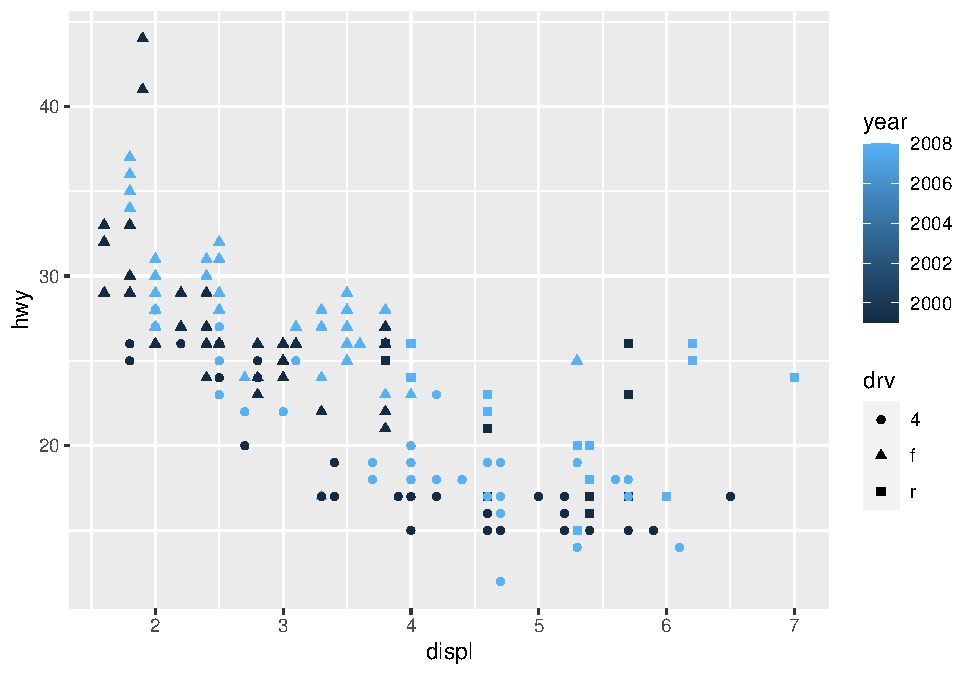
\includegraphics{Visualización-de-datos-con-ggplot2_files/figure-latex/unnamed-chunk-1-1.pdf}

El gráfico anterior nos deja observar que los vehículos con un mayor
volumen de motor, tienen en general un menor rendimiento de gasolina.

\begin{Shaded}
\begin{Highlighting}[]
\KeywordTok{ggplot}\NormalTok{(mpg) }\OperatorTok{+}
\StringTok{  }\KeywordTok{geom\_point}\NormalTok{(}\DataTypeTok{mapping =} \KeywordTok{aes}\NormalTok{(}\DataTypeTok{x =}\NormalTok{ displ, }\DataTypeTok{y =}\NormalTok{ hwy, }\DataTypeTok{colour =}\NormalTok{ cyl, }\DataTypeTok{shape =}\NormalTok{ drv)) }\OperatorTok{+}
\StringTok{  }\KeywordTok{geom\_smooth}\NormalTok{(}\DataTypeTok{mapping =} \KeywordTok{aes}\NormalTok{(}\DataTypeTok{x =}\NormalTok{ displ, }\DataTypeTok{y =}\NormalTok{ hwy), }\DataTypeTok{data =} \KeywordTok{filter}\NormalTok{( mpg, cyl }\OperatorTok{==}\StringTok{ }\DecValTok{4}\NormalTok{),}
              \DataTypeTok{colour=}\StringTok{"gold"}\NormalTok{) }\OperatorTok{+}
\StringTok{  }\KeywordTok{geom\_smooth}\NormalTok{(}\DataTypeTok{mapping =} \KeywordTok{aes}\NormalTok{(}\DataTypeTok{x =}\NormalTok{ displ, }\DataTypeTok{y =}\NormalTok{ hwy), }
              \DataTypeTok{data =} \KeywordTok{filter}\NormalTok{( mpg, cyl }\OperatorTok{==}\StringTok{ }\KeywordTok{c}\NormalTok{(}\DecValTok{4}\NormalTok{,}\DecValTok{5}\NormalTok{,}\DecValTok{6}\NormalTok{,}\DecValTok{8}\NormalTok{)),}
              \DataTypeTok{colour=}\StringTok{"royalblue"}\NormalTok{, }\DataTypeTok{se=}\NormalTok{F) }\OperatorTok{+}
\StringTok{  }\KeywordTok{geom\_smooth}\NormalTok{(}\DataTypeTok{mapping =} \KeywordTok{aes}\NormalTok{(}\DataTypeTok{x =}\NormalTok{ displ, }\DataTypeTok{y =}\NormalTok{ hwy),}
              \DataTypeTok{data =} \KeywordTok{filter}\NormalTok{( mpg, cyl }\OperatorTok{==}\StringTok{ }\DecValTok{6}\NormalTok{), }\DataTypeTok{colour=}\StringTok{"burlywood4"}\NormalTok{) }\OperatorTok{+}\StringTok{  }
\StringTok{  }\KeywordTok{geom\_smooth}\NormalTok{(}\DataTypeTok{mapping =} \KeywordTok{aes}\NormalTok{(}\DataTypeTok{x =}\NormalTok{ displ, }\DataTypeTok{y =}\NormalTok{ hwy),}
              \DataTypeTok{data =} \KeywordTok{filter}\NormalTok{( mpg, cyl }\OperatorTok{==}\StringTok{ }\DecValTok{8}\NormalTok{), }\DataTypeTok{colour=}\StringTok{"green"}\NormalTok{) }\OperatorTok{+}
\StringTok{  }\KeywordTok{facet\_wrap}\NormalTok{(}\OperatorTok{\textasciitilde{}}\NormalTok{year)}
\end{Highlighting}
\end{Shaded}

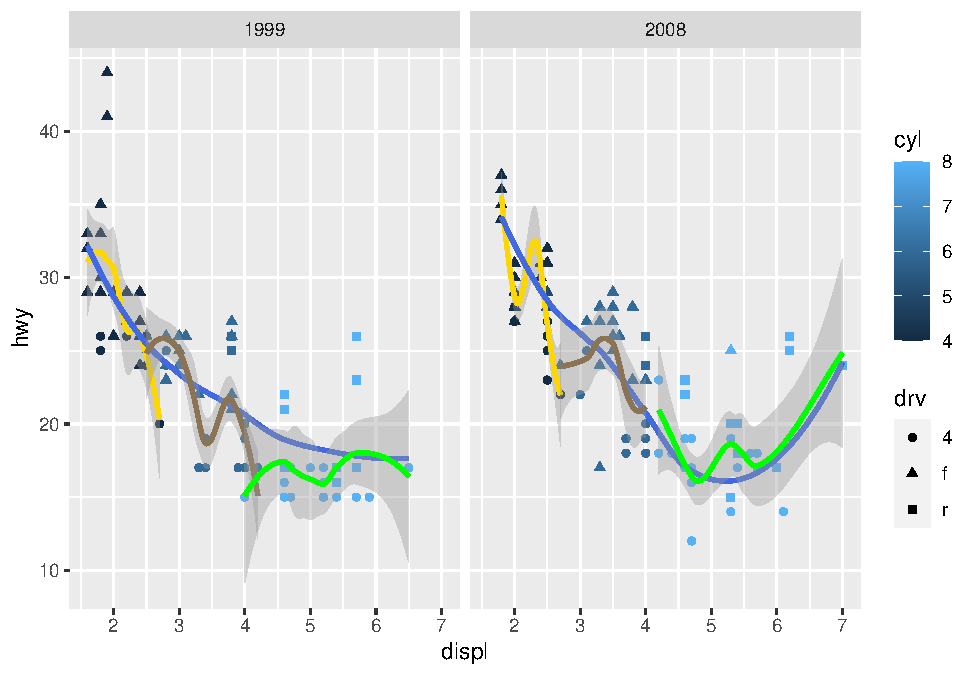
\includegraphics{Visualización-de-datos-con-ggplot2_files/figure-latex/unnamed-chunk-2-1.pdf}

El código anterior nos presenta dos gráficos, podemos ver la relación
entre los cilindros, parece ser que los autos con menor cilindraje
tienen mayor rendimiento (algo perceptible con el gráfico anterior, pues
a mayor volumen de motor, se usan mas cilindros).

Podemos ver más relaciones, por ejemplo los autos con mayor potencia,

\begin{Shaded}
\begin{Highlighting}[]
\KeywordTok{ggplot}\NormalTok{(mpg, }\DataTypeTok{mapping =} \KeywordTok{aes}\NormalTok{(}\DataTypeTok{x =}\NormalTok{ displ, }\DataTypeTok{y =}\NormalTok{ hwy)) }\OperatorTok{+}
\StringTok{  }\KeywordTok{geom\_point}\NormalTok{(}\DataTypeTok{mapping =} \KeywordTok{aes}\NormalTok{(}\DataTypeTok{colour =}\NormalTok{ class , }\DataTypeTok{shape =}\NormalTok{ fl)) }\OperatorTok{+}
\StringTok{  }\KeywordTok{geom\_smooth}\NormalTok{(}\DataTypeTok{data =} \KeywordTok{filter}\NormalTok{( mpg, cyl }\OperatorTok{==}\StringTok{ }\DecValTok{4}\NormalTok{), }\DataTypeTok{colour=}\StringTok{"gold"}\NormalTok{) }\OperatorTok{+}
\StringTok{  }\KeywordTok{geom\_smooth}\NormalTok{(}\DataTypeTok{data =} \KeywordTok{filter}\NormalTok{( mpg, cyl }\OperatorTok{==}\StringTok{ }\KeywordTok{c}\NormalTok{(}\DecValTok{4}\NormalTok{,}\DecValTok{5}\NormalTok{,}\DecValTok{6}\NormalTok{,}\DecValTok{8}\NormalTok{)), }
              \DataTypeTok{colour=}\StringTok{"royalblue"}\NormalTok{, }\DataTypeTok{se=}\NormalTok{F) }\OperatorTok{+}
\StringTok{  }\KeywordTok{geom\_smooth}\NormalTok{(}\DataTypeTok{data =} \KeywordTok{filter}\NormalTok{( mpg, cyl }\OperatorTok{==}\StringTok{ }\DecValTok{6}\NormalTok{), }\DataTypeTok{colour=}\StringTok{"burlywood4"}\NormalTok{) }\OperatorTok{+}\StringTok{  }
\StringTok{  }\KeywordTok{geom\_smooth}\NormalTok{(}\DataTypeTok{data =} \KeywordTok{filter}\NormalTok{( mpg, cyl }\OperatorTok{==}\StringTok{ }\DecValTok{8}\NormalTok{), }\DataTypeTok{colour=}\StringTok{"green"}\NormalTok{) }\OperatorTok{+}
\StringTok{  }\KeywordTok{facet\_wrap}\NormalTok{(}\OperatorTok{\textasciitilde{}}\NormalTok{year)}
\end{Highlighting}
\end{Shaded}

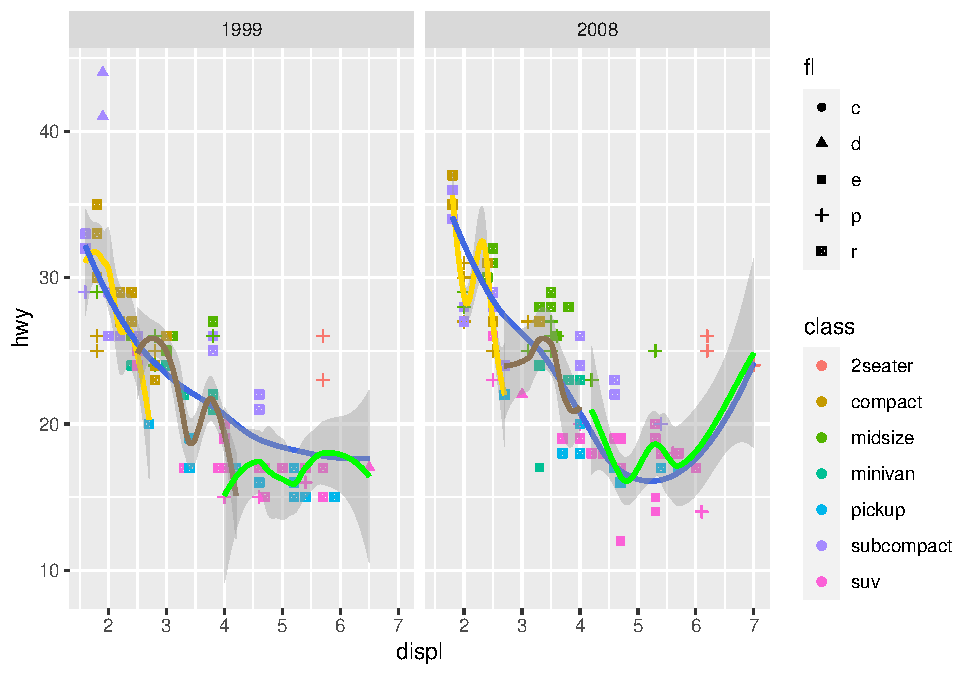
\includegraphics{Visualización-de-datos-con-ggplot2_files/figure-latex/unnamed-chunk-3-1.pdf}

las posibilidades son bastantes, aunque este dataset esta muy limitado.
por ello cambiaremos a uno con una cantidad bastante superior de datos.

\hypertarget{diamantes}{%
\subsection{Diamantes}\label{diamantes}}

El dataset diamonds cuenta con una muestra de 53940 diamantes.

\begin{itemize}
\item
  Las Variables

  \begin{itemize}
  \tightlist
  \item
    price

    \begin{itemize}
    \tightlist
    \item
      price in US dollars (\$326--\$18,823)
    \end{itemize}
  \item
    carat

    \begin{itemize}
    \tightlist
    \item
      weight of the diamond (0.2--5.01)
    \end{itemize}
  \item
    cut

    \begin{itemize}
    \tightlist
    \item
      quality of the cut (Fair, Good, Very Good, Premium, Ideal)
    \end{itemize}
  \item
    color

    \begin{itemize}
    \tightlist
    \item
      diamond colour, from D (best) to J (worst)
    \end{itemize}
  \item
    clarity

    \begin{itemize}
    \tightlist
    \item
      a measurement of how clear the diamond is (I1 (worst), SI2, SI1,
      VS2, VS1, VVS2, VVS1, IF (best))
    \end{itemize}
  \item
    x

    \begin{itemize}
    \tightlist
    \item
      length in mm (0--10.74)
    \end{itemize}
  \item
    y

    \begin{itemize}
    \tightlist
    \item
      width in mm (0--58.9)
    \end{itemize}
  \item
    z

    \begin{itemize}
    \tightlist
    \item
      depth in mm (0--31.8)
    \end{itemize}
  \item
    depth

    \begin{itemize}
    \tightlist
    \item
      total depth percentage = z / mean(x, y) = 2 * z / (x + y) (43--79)
    \end{itemize}
  \item
    table
  \item
    width of top of diamond relative to widest point (43--95)
  \end{itemize}
\end{itemize}

\begin{Shaded}
\begin{Highlighting}[]
\KeywordTok{ggplot}\NormalTok{(diamonds) }\OperatorTok{+}
\StringTok{  }\KeywordTok{geom\_bar}\NormalTok{(}\DataTypeTok{mapping =} \KeywordTok{aes}\NormalTok{(}\DataTypeTok{x =}\NormalTok{ cut, }\DataTypeTok{colour =}\NormalTok{ cut)) }\OperatorTok{+}
\StringTok{  }\KeywordTok{stat\_count}\NormalTok{(}\DataTypeTok{mapping =}  \KeywordTok{aes}\NormalTok{(}\DataTypeTok{x=}\NormalTok{cut))}
\end{Highlighting}
\end{Shaded}

\includegraphics{Visualización-de-datos-con-ggplot2_files/figure-latex/unnamed-chunk-4-1.pdf}
\# Esteticas

Aprenderemos el uso de las estéticas con los siguientes ejemplos.

\begin{Shaded}
\begin{Highlighting}[]
\KeywordTok{ggplot}\NormalTok{(diamonds, }\DataTypeTok{mapping =} \KeywordTok{aes}\NormalTok{(}\DataTypeTok{x =}\NormalTok{ cut, }\DataTypeTok{fill =}\NormalTok{ clarity )) }\OperatorTok{+}
\StringTok{  }\KeywordTok{geom\_bar}\NormalTok{(}\DataTypeTok{position =} \StringTok{"identity"}\NormalTok{) }\OperatorTok{+}
\StringTok{  }\KeywordTok{geom\_bar}\NormalTok{(}\KeywordTok{aes}\NormalTok{(}\DataTypeTok{colour=}\NormalTok{clarity), }\DataTypeTok{alpha =} \FloatTok{.5}\NormalTok{) }
\end{Highlighting}
\end{Shaded}

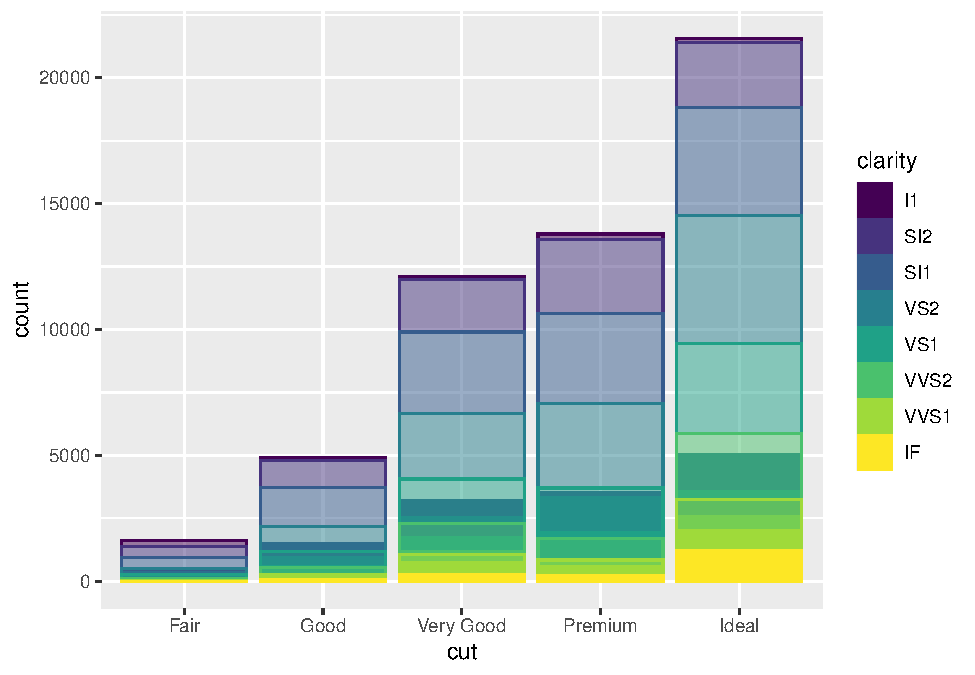
\includegraphics{Visualización-de-datos-con-ggplot2_files/figure-latex/unnamed-chunk-5-1.pdf}

Quizá el anterior gráfico a simple vista no nos ayude mucho a entender
lo que hace la estética \texttt{position="identity"}, eso es debido a
que es un gráfico de barras, pero aquí se muestra con una claridad
superior\footnote{El problema de nombres en los ejes será tratado mas
  adelante.} que esta estética se encarga de no apilar, sino simplemente
colocar la medida exacta de los datos, notemos que la acumulación en
ideal es bastante mayor a los 20000 en el gráfico apilado, mientras en
el de identity, apenas llega sobre los 5000.

\begin{Shaded}
\begin{Highlighting}[]
\KeywordTok{ggplot}\NormalTok{(diamonds, }\DataTypeTok{mapping =} \KeywordTok{aes}\NormalTok{(}\DataTypeTok{x =}\NormalTok{ cut, }\DataTypeTok{fill =}\NormalTok{ clarity, }\DataTypeTok{colour =}\NormalTok{ cut, }\DataTypeTok{xlab =}\NormalTok{ F )) }\OperatorTok{+}
\StringTok{  }\KeywordTok{geom\_bar}\NormalTok{() }\OperatorTok{+}
\StringTok{  }\KeywordTok{facet\_grid}\NormalTok{(}\OperatorTok{\textasciitilde{}}\NormalTok{clarity)}
\end{Highlighting}
\end{Shaded}

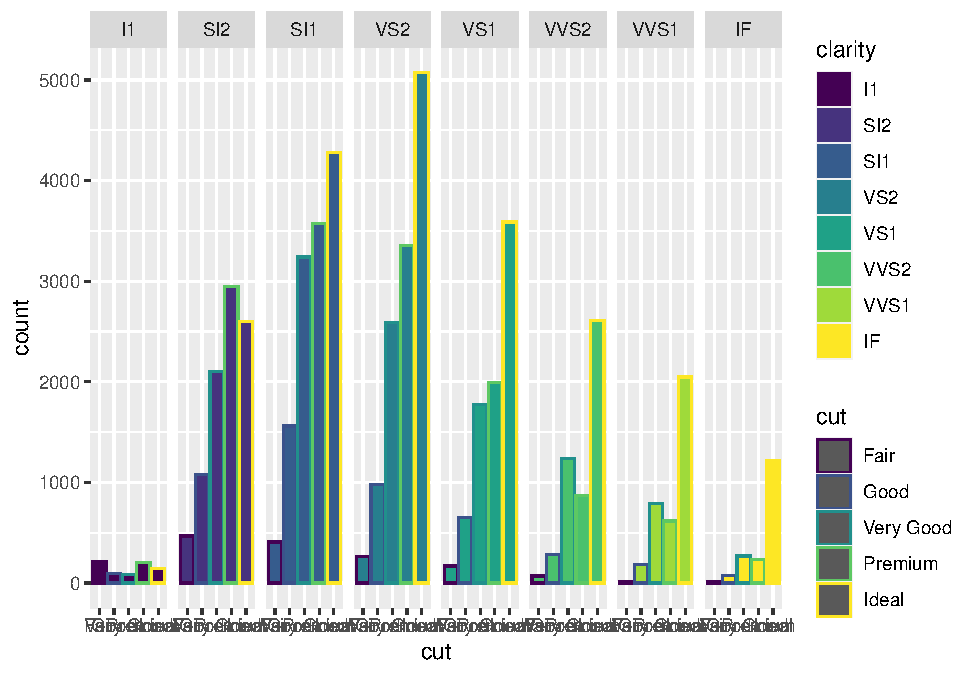
\includegraphics{Visualización-de-datos-con-ggplot2_files/figure-latex/unnamed-chunk-6-1.pdf}

\hypertarget{position-fill}{%
\paragraph{\texorpdfstring{\texttt{position\ =\ "fill"}}{position = "fill"}}\label{position-fill}}

\begin{Shaded}
\begin{Highlighting}[]
\KeywordTok{ggplot}\NormalTok{(diamonds, }\DataTypeTok{mapping =} \KeywordTok{aes}\NormalTok{(}\DataTypeTok{x =}\NormalTok{ cut, }\DataTypeTok{fill =}\NormalTok{ clarity )) }\OperatorTok{+}
\StringTok{  }\KeywordTok{geom\_bar}\NormalTok{(}\DataTypeTok{position =} \StringTok{"fill"}\NormalTok{) }\OperatorTok{+}
\StringTok{  }\KeywordTok{geom\_bar}\NormalTok{(}\KeywordTok{aes}\NormalTok{(}\DataTypeTok{colour=}\NormalTok{clarity), }\DataTypeTok{alpha =} \FloatTok{.5}\NormalTok{) }
\end{Highlighting}
\end{Shaded}

\begin{center}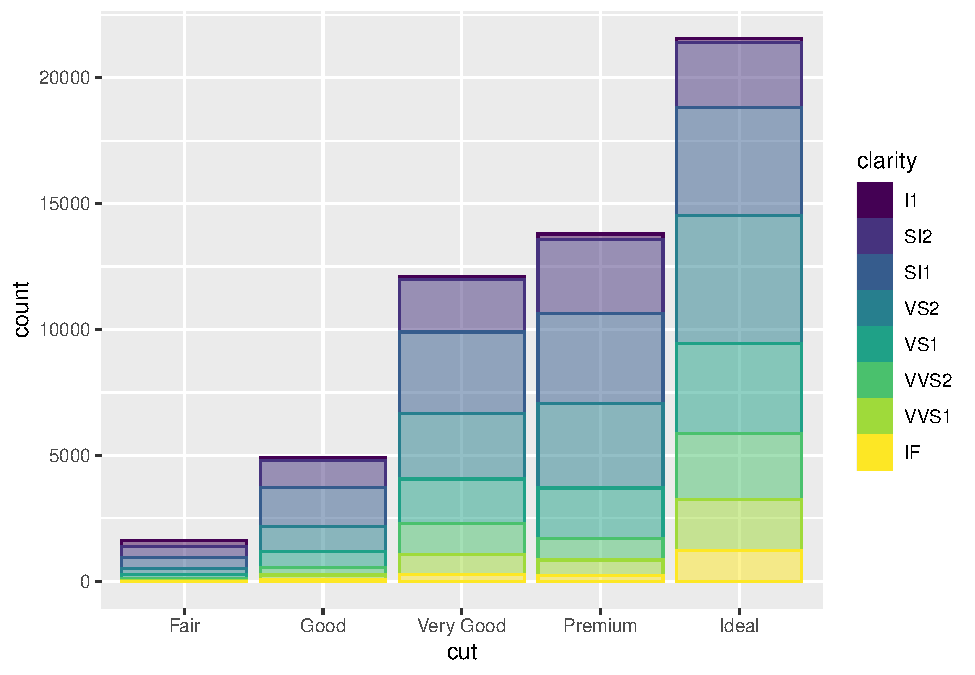
\includegraphics{Visualización-de-datos-con-ggplot2_files/figure-latex/unnamed-chunk-7-1} \end{center}

para resolverlos necesitas hacer en este caso una pequeña factorización.
o sea que metes todo lo que se vea igual dentro de un parentesis y usas
la propiedad de distribución de los números reales. Y en estos casos
particulares, tienes que pensar cuando un numero da cero. por ejemplo,
si multiplicas cualquier número por 0, te va a dar 0, entonces tienes
que volver en cero los números en la factorización.

\end{document}
